% %-----------------------------------------------------------------------------%
\begin{landscape}
\addappendix{Diagram Ekstraksi Fitur}
\chapter*{Lampiran 1: Diagram Ekstraksi Fitur}
\label{Lampiran 1: Diagram Ekstraksi Fitur}
\begin{figure}
    \centering
    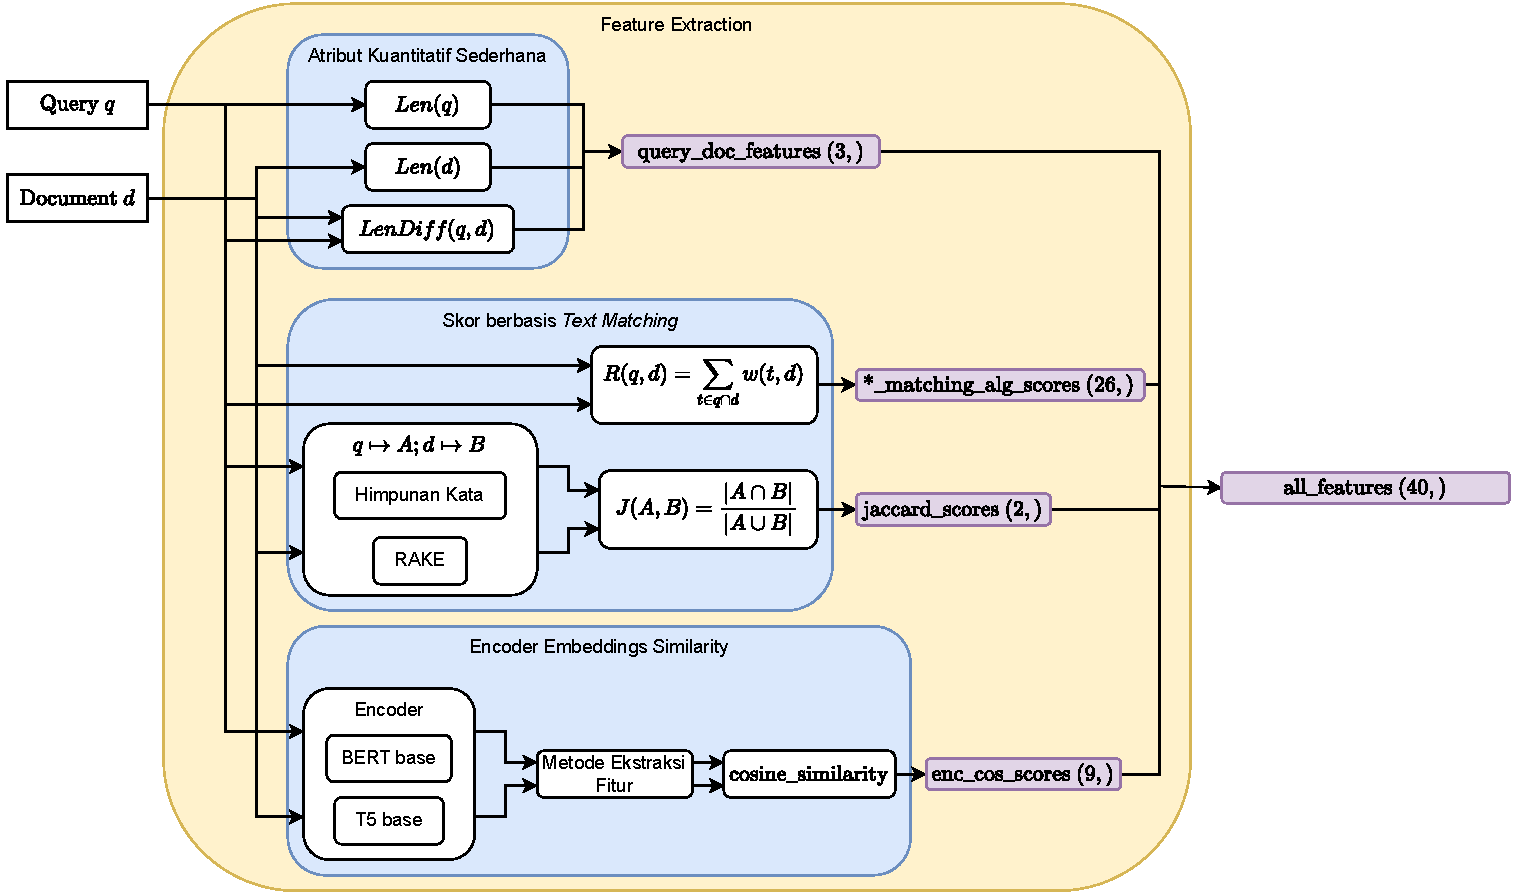
\includegraphics[scale=0.75]{assets/pdfs/ekstraksiFitur.pdf}
    \caption{Diagram ekstraksi fitur. Perhatikan bahwa warna ungu menandakan nama variabel yang diimplementasikan pada \bab{}~\ref{bab:4} dengan tambahan informasi dimensi vektor atau jumlah fitur yang diperoleh.}
    \label{fig:diagramEkstraksiFitur}
\end{figure}
\end{landscape}
% %-----------------------------------------------------------------------------%
% \todo{Silakan hapus lampiran ini ketika Anda mulai menggunakan \f{template}.}

% \f{Template} versi terbaru bisa didapatkan di \url{https://gitlab.com/ichlaffterlalu/latex-skripsi-ui-2017}.
% Daftar perubahan pada \f{template} hingga versi ini:
% \begin{itemize}
% 	\item versi 1.0.3 (3 Desember 2010):
% 		\begin{itemize}
% 			\item \f{Template} Skripsi/Tesis sesuai ketentuan \f{formatting} tahun 2008.
% 			\item Bisa diakses di \url{https://github.com/edom/uistyle}.
% 		\end{itemize}
% 	\item versi 2.0.0 (29 Januari 2020):
% 		\begin{itemize}
% 			\item \f{Template} Skripsi/Tesis sesuai ketentuan \f{formatting} tahun 2017.
% 			\item Menggunakan BibTeX untuk sitasi, dengan format \f{default} sitasi IEEE.
% 			\item \f{Template} kini bisa ditambahkan kode sumber dengan \f{code highlighting} untuk bahasa pemrograman populer seperti Java atau Python.
% 		\end{itemize}
% 	\item versi 2.0.1 (8 Mei 2020):
% 		\begin{itemize}
% 			\item Menambahkan dan menyesuaikan tutorial dari versi 1.0.3, beserta cara kontribusi ke template.
% 		\end{itemize}
% 	\item versi 2.0.2 (14 September 2020):
% 		\begin{itemize}
% 			\item Versi ini merupakan hasil \f{feedback} dari peserta skripsi di lab \f{Reliable Software Engineering} (RSE) Fasilkom UI, semester genap 2019/2020.
% 			\item BibTeX kini menggunakan format sitasi APA secara \f{default}.
% 			\item Penambahan tutorial untuk \code{longtable}, agar tabel bisa lebih dari 1 halaman dan header muncul di setiap halaman.
% 			\item Menambahkan tutorial terkait penggunaan BibTeX dan konfigurasi \f{header}/\f{footer} untuk pencetakan bolak-balik.
% 			\item Label "Universitas Indonesia" kini berhasil muncul di halaman pertama tiap bab dan di bagian abstrak - daftar kode program.
% 			\item \f{Hyphenation} kini menggunakan \code{babel} Bahasa Indonesia. Aktivasi dilakukan di \code{hype-indonesia.tex}.
% 			\item Minor adjustment untuk konsistensi \f{license} dari template.
% 		\end{itemize}
% 	\item versi 2.0.3 (15 September 2020):
% 		\begin{itemize}
% 			\item Menambahkan kemampuan orientasi \f{landscape} beserta tutorialnya.
% 			\item \code{\bslash{}captionsource} telah diperbaiki agar bisa dipakai untuk \code{longtable}.
% 			\item Daftar lampiran kini telah tersedia, lampiran sudah tidak masuk daftar isi lagi.
% 			\item Nomor halaman pada lampiran dilanjutkan dari halaman terakhir konten (daftar referensi).
% 			\item Kini sudah bisa menambahkan daftar isi baru untuk jenis objek tertentu (custom), seperti: "Daftar Aturan Transformasi".
% 			Sudah termasuk mekanisme \f{captioning} dan tutorialnya.
% 			\item Perbaikan minor pada tutorial.
% 		\end{itemize}
% 	\item versi 2.1.0 (8 September 2021):
% 		\begin{itemize}
% 			\item Versi ini merupakan hasil \f{feedback} dari peserta skripsi dan tesis di lab \f{Reliable Software Engineering} (RSE) Fasilkom UI, semester genap 2020/2021.
% 			\item Minor edit: "Lembar Pengesahan", dsb. di daftar isi menjadi all caps.
% 			\item Experimental multi-language support (Chinese, Japanese, Korean).
% 			\item Support untuk justifikasi dan word-wrapping pada tabel.
% 			\item Penggunaan suffix "(sambungan)" untuk tabel lintas halaman. Tambahan support suffix untuk \code{\bslash{}captionsource}.
% 		\end{itemize}
% 	\item versi 2.1.1 (7 Februari 2022):
% 		\begin{itemize}
% 			\item Update struktur mengikuti fork template versi 1.0.3 di \url{https://github.com/rkkautsar/edom/ui-thesis-template}.
% 			\item Support untuk simbol matematis \code{amsfonts}.
% 			\item Kontribusi komunitas terkait improvement GitLab CI, atribusi, dan format sitasi APA bahasa Indonesia.
% 			\item Perbaikan tutorial berdasarkan perubahan terbaru pada versi 2.1.0 dan 2.1.1.
% 		\end{itemize}
% 	\item versi 2.1.2 (13 Agustus 2022):
% 		\begin{itemize}
% 			\item Modifikasi penamaan beberapa berkas.
% 			\item Perbaikan beberapa halaman depan (halaman persetujuan, halaman orisinalitas, dsb.).
% 			\item Support untuk lembar pengesahan yang berbeda dengan format standar, seperti Laporan Kerja Praktik dan Disertasi.
% 			\item Kontribusi komunitas terkait kesesuaian dengan format Tugas Akhir UI, kelengkapan dokumen, perbaikan format sitasi, dan \f{quality-of-life}.
% 			\item Perbaikan tutorial.
% 		\end{itemize}
% 	\item versi 2.1.3 (22 Februari 2023):
% 		\begin{itemize}
% 			\item Dukungan untuk format Tugas Akhir Kelompok di Fasilkom UI.
% 			\item Dukungan untuk format laporan Kampus Merdeka Mandiri di Fasilkom UI.
% 			\item Minor bugfix: Perbaikan kapitalisasi variabel.
% 			\item Quality-of-Life: Pengaturan kembali \code{config/settings.tex}.
% 			\item Tutorial untuk beberapa \f{use case}.
% 		\end{itemize}
% \end{itemize}

% %-----------------------------------------------------------------------------%
% \addappendix{Judul Lampiran 2}
% \chapter*{Lampiran 2: Judul Lampiran 2}
% \label{appendix:sample}
% %-----------------------------------------------------------------------------%
% Lampiran hadir untuk menampung hal-hal yang dapat menunjang pemahaman terkait tugas akhir, namun akan mengganggu \f{flow} bacaan sekiranya dimasukkan ke dalam bacaan.
% Lampiran bisa saja berisi data-data tambahan, analisis tambahan, penjelasan istilah, tahapan-tahapan antara yang bukan menjadi fokus utama, atau pranala menuju halaman luar yang penting.

% %-----------------------------------------------------------------------------%
% \section*{Subbab dari Lampiran 2}
% \label{appendix:sampleSubchap}
% %-----------------------------------------------------------------------------%
% \todo{Isi subbab ini sesuai keperluan Anda. Anda bisa membuat lebih dari satu judul lampiran, dan tentunya lebih dari satu subbab.}
